\section{Theory}

\subsection{Haplogroups}

The human Y chromosome is only inherited from father to
son. Usually large parts of it are unchanged but sometimes
a mutation at a single position occurs. Such mutations are
called SNPs (Single Nucleotide Polymorphisms). They are
very stable and can be used to group people into ancestral
lines.

\begin{figure}[ht]
\centering
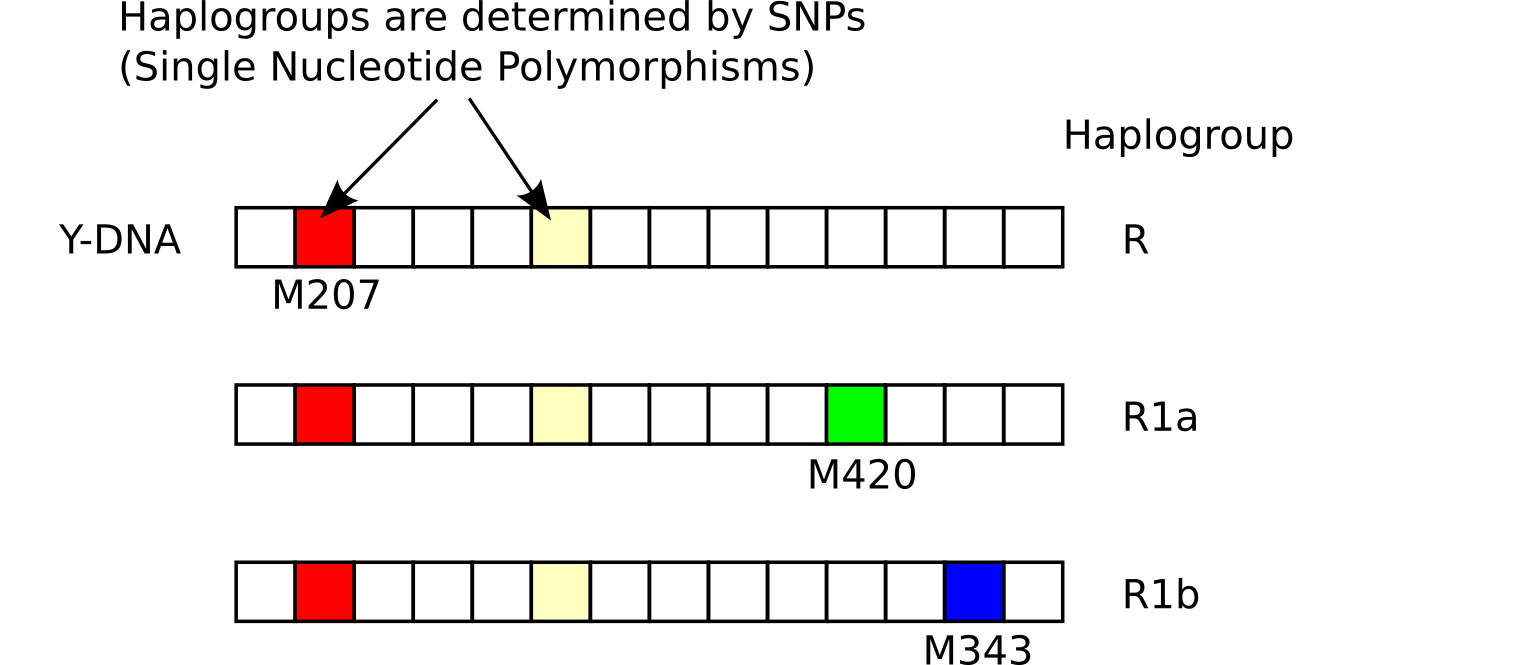
\includegraphics[width=13cm]{img/haplogroups.png}
\caption{\label{haplogroup} A set of single mutations
defines a person's haplogroup. Persons who belong to the
same haplogroup usually share a common ancestor within a
few thousand years.}
\end{figure}

Figure \ref{haplogroup} illustrates a typical situation.
Many Europeans belong to haplogroup R, which is characterized
by the mutation M207 and others which are not mentioned here.
The M207 marker is inherited throughout all following ancestral
lines. Later the mutations M420 and M343 occurred. They are
mutually exclusive to each other thus defining separate
lineages. The marker M420 defines the haplogroup R1a which
is common in Eastern Europe and the marker M343 defines the
haplogroup R1b which is common in Western Europe. Because
all people who belong to R1a and R1b share the M207 marker
we know that they also share a common ancestor a long time
ago.

SNPs do not occur very often. Persons who belong to the
same haplogroup usually share a common ancestor within a
few thousand years. If you know your haplogroup it will
tell you something about your deep history (thousands
of years).


\subsection{Haplotypes}

Most people want to know more about family relationships.
Luckily there is another type of mutations that occurs much
more often than SNPs. This is the repetition of certain
genetic patterns. They group people into haplotypes.

\begin{figure}[ht]
\centering
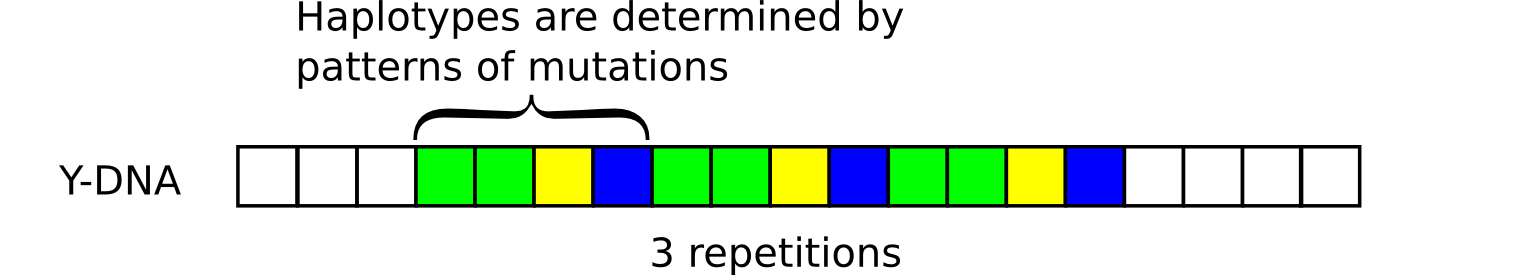
\includegraphics[width=13cm]{img/haplotypes.png}
\caption{\label{haplotype} A person's haplotype is defined
by patterns of mutations. Persons with the same haplotype
usually share a common ancestor within a few hundred years
if they take a standard test with 37 markers or more.}
\end{figure}

On the Y chromosome there are many different patterns that
repeat themselves. Every pattern has a name, for example DYS393.
If we count the number of repetitions for a specific pattern
we get a value, for example DYS393=13. Figure \ref{haplotype}
illustrates the situation for an exemplary marker. The pattern
is repeated 3 times. So this marker has a value of 3.

If a mutation occurs the number of repetitions changes. A 
single marker mutates rarely but the modern standard tests
use many markers at the same time, most often 37, 67 or
111. The combination of all these markers defines
a haplotype. Persons who share the same haplotype usually
also share a common ancestor within a few hundred years.

It is important to realize that haplotypes are not as good
as haplogroups. Haplotypes sometimes overlap between separate
lineages. So when working with haplotypes the haplogroup
should also be known.

Phylofriend uses haplotypes to calculate genetic distances
between persons by counting the number of different mutations.


\subsection{Phylogenetic Trees}

Phylogenetic trees group people together according to their
genetic distances. They give us a picture of how different
persons are related.

\begin{figure}[ht]
\centering
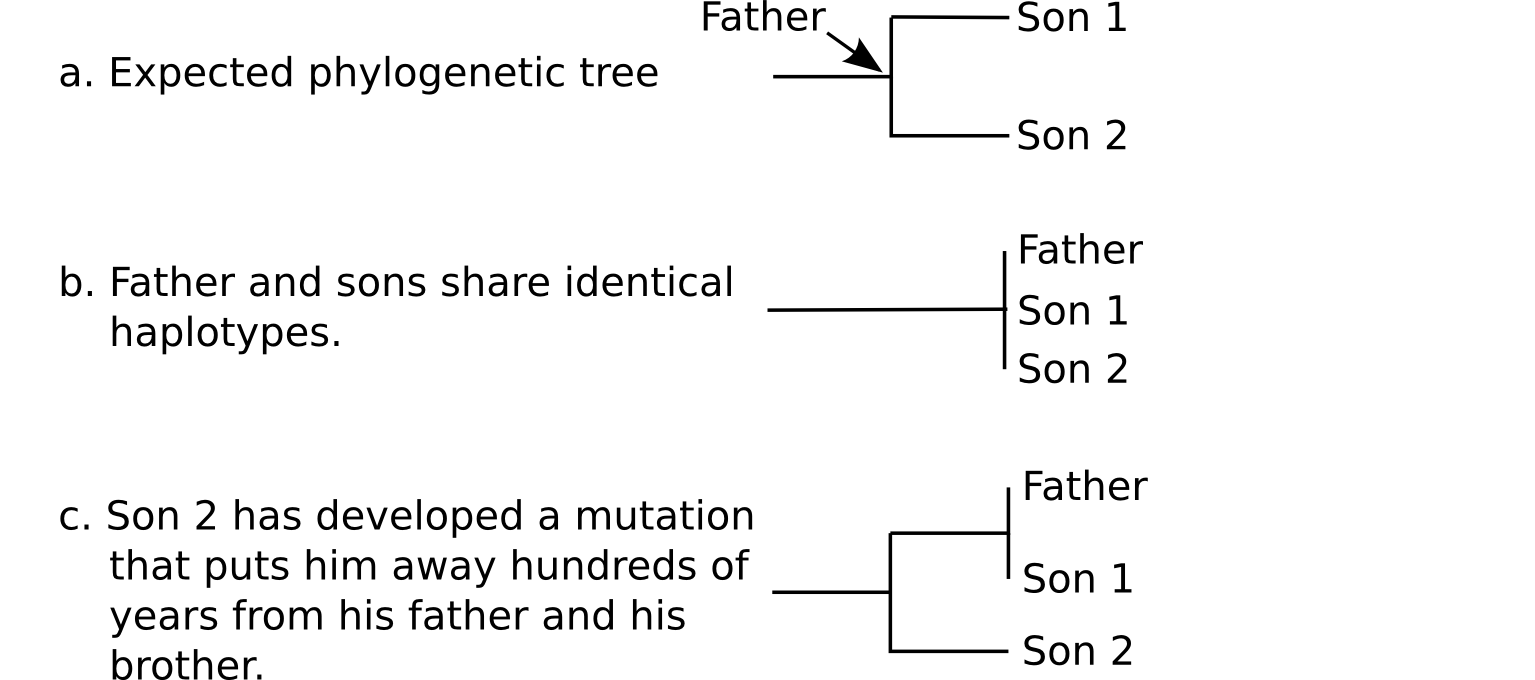
\includegraphics[width=13cm]{img/phylotrees.png}
\caption{\label{phylotrees} Phylogenetic trees group persons
together according to their genetic distances. Genetic
distances are often associated with time scales but this
is only true for long time spans.}
\end{figure}

Figure \ref{phylotrees} shows some exemplary trees. If a
father has two sons we would expect that both sons are at
a little genetic distance away from their father. If they
are not twins they also should be separated by each other.
Tree a illustrates this situation. This is exactly the
tree we would get if we could measure the genetic distance
at a high resolution and know the birth dates of father and
sons. Because we know the birth dates we would put the father
before the sons and associate the horizontal axis with a
time scale assuming that genetic distance is proportional
to time.

Reality however shows a different picture. The currently
available standard tests (37, 67 and 111 markers) only offer
a low resolution. So most often we can not measure any genetic
distance between father and sons. This is illustrated by
tree b. Because the tree illustrates genetic distances and
not time distances father and sons are all side by side.

If son 2 develops a mutation by chance we get a confusing picture.
Son 2 is suddenly far away from his father and his brother.
This is shown by tree c. The reason for the great distance
between father and son 2 is the low resolution of the test.
If we take the mutation rates from \cite{Kly12} we can
calculate how long it takes on average for a mutation to
occur. For a 37 marker test the result is 280 years, for
a 67 marker test 210 years and for a 111 marker test 130
years. 

This means if the father and his sons took a 37 marker test
and son 2 has developed a mutation by chance he will appear
to be 280 years away from his father but the only reason for
that is the low resolution of the test.

In most cases the standard tests are good enough. We do not
need a paternity test for genealogical purposes but it is
important to remember that the standard tests only places
persons into time frames of hundreds of years.




